% contient une explication du fonctionnement du Mip Map et du Rip Map, et des schémas explicatifs. En bref, un résumé de l'article de Williams
% parler éventuellement de la méthode naïve, ou d'autres méthodes actuelles qui ne fonctionnent pas

A few methods have been developed to process homographies. There are inspired by the Mipmap method presented by Williams in 1983 \cite{williams1983pyramidal}. This section presents the Mipmap and one of its alternative, the Ripmap. In the Experiments section it is compared to the new method.

  %Afin de traiter les homographies plusieurs méthodes ont été développées. Elles sont pour la plupart des variantes de Mipmap présentée par Williams en 1983 \cite{williams1983pyramidal}. Cette partie présente le Mipmap et le Ripmap. Le Ripmap comparé avec la nouvelle méthode dans les expériences.

\sse{Presentation of the Mipmap}
\label{Mipmap}
The principle of the Mipmap method is to precompute local averaging of the input image at different scale, in order to compute an homography in real-time. To reach this goal it is assumed that the input image is a square with size a power of two.

Then the average square of four pixels is compute to obtain a square two times smaller. This process is then iterate to build a sequence of images, each one being two times smaller than the previous one. An example of Mipmap is represented figure \ref{MipMap_real}.

%\sse{Présentation du Mipmap}
%\label{Mipmap}
%Le principe du Mipmap est de précalculer des  moyennes locales de l'image à plusieurs échelles, pour pouvoir ensuite calculer en temps réel une homographie. 

%Pour cela on choisit de supposer que l'image est carrée de taille une puissance de 2 (quitte à faire un premier zoom). On calcule ensuite la valeur moyenne de certains carrés de l'image de taille une puissance de 2.
%Le Mipmap est donc représenté par une suite d'images chacune deux fois plus petite que la précédente. Ainsi c'est un suite de \emph{zoom-out} de l'image d'origine de facteur une puissance de 2. 

%Un exemple est représenté figure \ref{MipMap_real}.

\label{exemple_de_mipmap_figure}
\begin{figure}[h!]
\centering
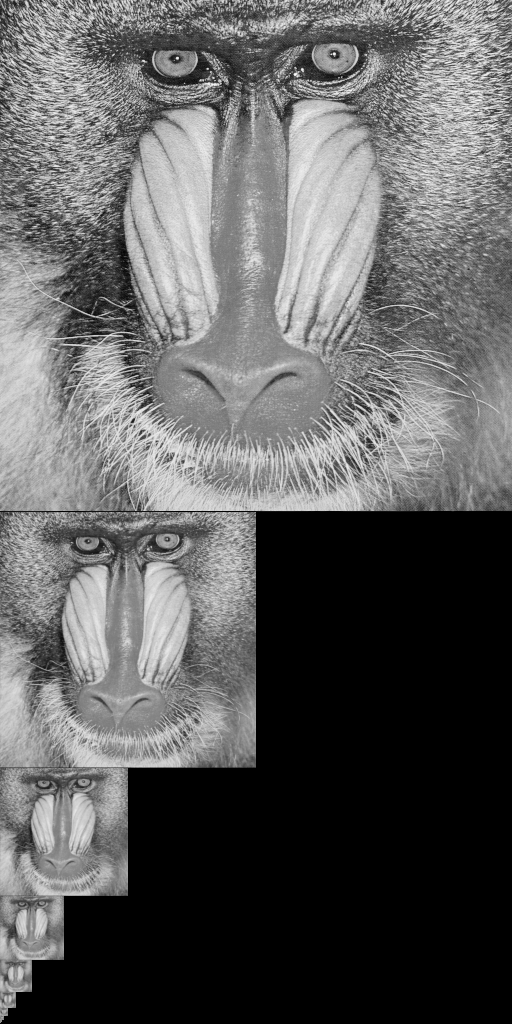
\includegraphics[scale=0.4]{MipMap_real} %scale=0.4 ça fait vachement petit, non ?
\caption{An example of Mipmap (cf. section \ref{exemple_de_mipmap_figure})}
\label{MipMap_real}
\end{figure}

To compute the value of a pixel of the output image, the area of the input image corresponding is approximated by using the differential of the inverse homography. Then the parallelogram obtained is approximate by squares.

The size of the approximation square is called distance since the "farer" a pixel is, the bigger the squares that approximate it are.

Assume there is a formula giving the distance of any points. The geometry of the Mipmap only allowed distances power of two, so a new interpolation scheme is required. It is the trilinear interpolation :

\begin{itemize}
\item On one hand, there is a linear interpolate between two level of the Mipmap
\item On the other hand in each level there is a bilinear interpolation.
\end{itemize}

The Figure \ref{intertrilineaire} represent this interpolation.

%Quand on cherche la valeur d'un pixel de l'image d'arrivée, on approche la zone de l'image de départ à laquelle il correspond à l'aide de la différentielle de l'homographie inverse. On obtient alors un parallélogramme, qu'on essaye d'approcher avec des carrés. 

%On appelle distance d'un pixel la taille du carré choisi pour l'approximation (car plus un pixel est "loin", plus les carrés qui l'approchent sont grands). 

%On suppose que l'on dispose d'une formule qui nous donne la distance d'un point quelconque. La géométrie du Mipmap ne permettant que des distances puissance de 2, on fait une approximation trilinéaire : 

%\begin{itemize}
  %\item d'une part, on fait une interpolation linéaire entre deux étages dont les profondeurs encadrent la distance.
 % \item d'autre part, dans chaque étage du Mipmap, on fait une interpolation bilinéaire entre les quatre carrés qui encadrent le pixel.
%\end{itemize}

%La figure \ref{intertrilineaire} schématise cette interpolation. 

\label{figure_schema_inter_trilin}
\begin{figure}[h!]
\centering
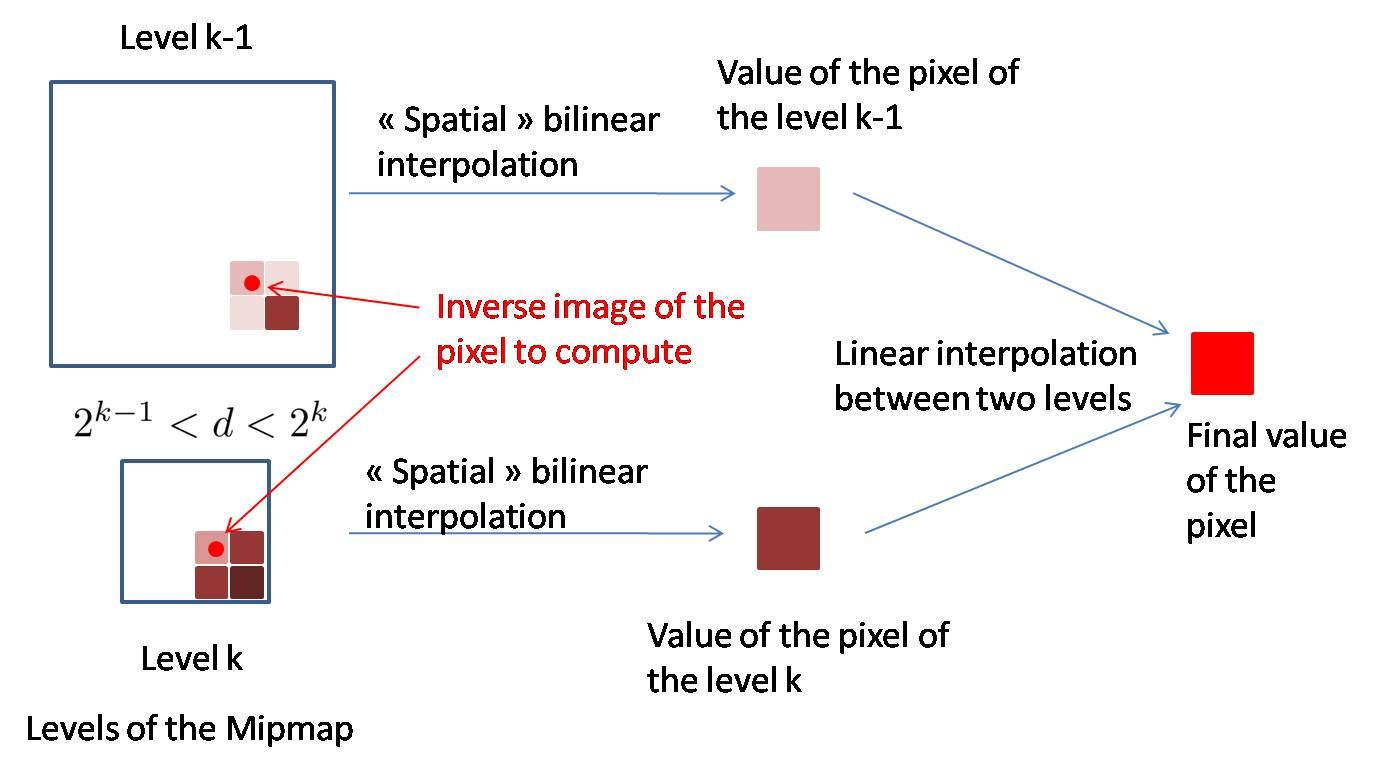
\includegraphics[scale=0.5]{intertrilineaire.jpg}
\caption{Trilinear interpolation (cf. section \ref{figure_schema_inter_trilin})}
\label{intertrilineaire}
\end{figure}

\sse{Distance function}
\label{fonctiondistance}

The choice of the distance function is now discussed. It is a crucial point in the Mipmap method because if the distance $d$ is too large, the image is over blurred, and if it is too small the image is aliased.

Every distance function is build using the differential of the inverse homographs. Let $(u,v)$ be the coordinate in the input image and $(x,y)$ the coordinate in the output image. Let $H$ be the inverse homography, then $(u,v)=H(x,y)$. $\frac{\dr u}{\dr x}$ is the partial derivative of $u$ with respect to $x$

A few distance have been tried, finally we choose the larger side method.

%\sse{Les fonctions de distance}
%\label{fonctiondistance}

%On a supposer l'existence d'une fonction qui a un point associe une distance, on va maintenant s'intéresser au fonctions possibles.

%Le choix de la distance est crucial car si $d$ est trop grand, l'image est inutilement floutée (on parle d'\emph{over-blurring}), et si $d$ est trop petit, l'image est aliasée.

Toutes les fonctions de distance dépendent de la différentielle de l'homographie inverse.
On note $(u,v)$ les coordonnées dans l'image d'origine et $(x,y)$ celles dans la fenêtre d'arrivée.

Il est aisé de calculer les coefficients des dérivées partielles. On note $H$ l'homographie inverse.

%re image prgm, avec les dérivé partielle indiqués

% On a jugé de la performance des méthodes "à vue". On compte à terme l'évaluer sur des cosinus/sinus.

%On a ainsi $(u,v)=H(x,y)$, et on note par exemple $\frac{\dr u}{\dr x}$ la dérivée partielle de $u$ par rapport à $x$.

%On donne ici sa formule.

$$ D(x,y) = \max \left(\sqrt{\left(\frac{\dr u}{\dr x}\right)^2 + \left(\frac{\dr v}{\dr x}\right)^2},\sqrt{\left(\frac{\dr u}{\dr y}\right)^2 + \left(\frac{\dr v}{\dr y}\right)^2}\right)$$

The distance is the larger side of the parallelogram. This formula is from an article by Heckbert \cite{heckbert1983texture}. It is represented figure \ref{methode_plus_grand_cote}.

%On prend le plus grand côté du parallélogramme comme côté du carré. Cette formule vient d'un article de Heckbert \cite{heckbert1983texture}. On la représente figure \ref{methode_plus_grand_cote}.

\begin{figure}[h!]
\centering
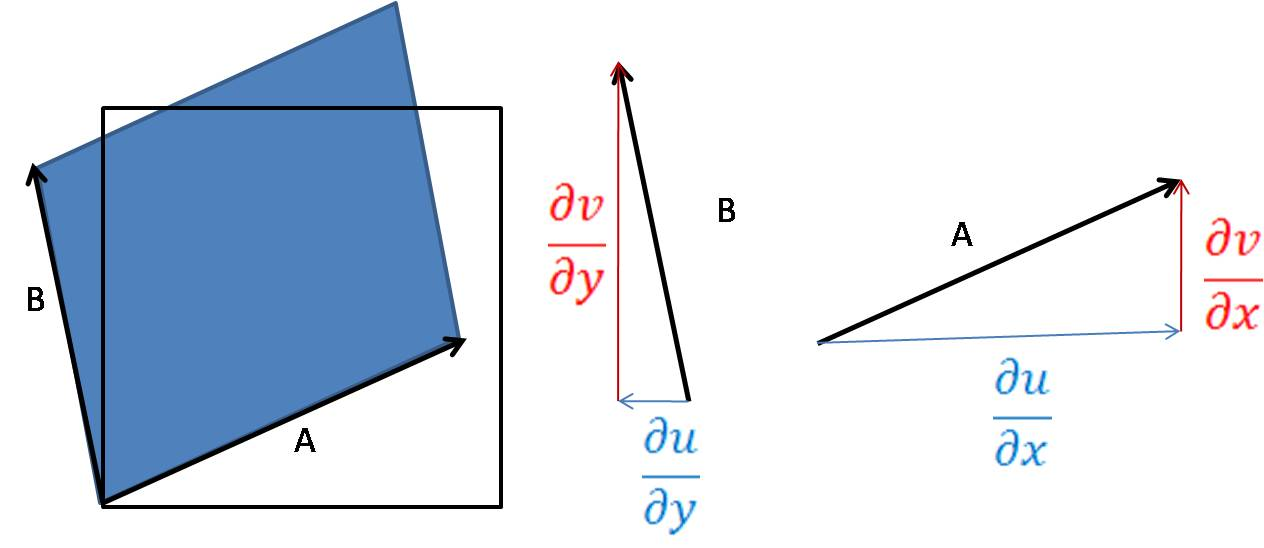
\includegraphics[scale=0.5]{methode_plus_grand_cote.jpg}
\caption{Larger side method (there it is A)}
\label{methode_plus_grand_cote}
\end{figure}


\sse{An improved algorithm : the Ripmap}
\label{Ripmap}

On of the great weakness of the Mipmap is its isotropy. In fact if the parallelogram to approximate is a flat rectangle there is no reasonable approximation with a square.

To palliate this problem the Ripmap is used \cite{akenine2008real}. This is a Mipmap where the average  of all the rectangles of width and height a power of two has also been precompute. There is an example of Ripmap figure \ref{Ripmap_real}, and two algorithms to build one in appendix in \ref{pseudo_code_Ripmap}. The algorithm \ref{buildRipmap1} is naive, the real implementation use the algorithm \ref{buildRipmap2} which convolve images with a gaussian before each down-sampling.

The distance function return two values, one for each side of the rectangle. Then a quadri-linear interpolation is compute (bilinear between the level and bilinear inside each level). This interpolation scheme is represented figure \ref{interbibilineaire}. The algorithm \ref{interbibi1} in appendix in \ref{pseudo_code_Ripmap} describe this interpolation.




%\sse{Algorithme amélioré : Le Ripmap}
%\label{Ripmap}
%Une des grandes faiblesses du Mipmap est l'isotropie : il ne privilégie aucune direction. Ainsi si le parallélogramme à approcher est un rectangle très plat, il n'y a pas d'approximation raisonnable à l'aide d'un carré.

%Pour tenter de résoudre ce problème on utilise le Ripmap \cite{akenine2008real}. C'est en fait un Mipmap où l'on a aussi calculé la moyenne de tous les rectangles dont les côtés sont des puissances de deux. Un exemple est présenté dans la figure \ref{Ripmap_real}, ainsi que deux algorithmes de construction en annexe en \ref{pseudo_code_Ripmap}. L'algorithme \ref{buildRipmap1} est naïf, en pratique c'est l'algorithme \ref{buildRipmap2} qui est implémenté, il convole par une gaussienne avant chaque sous-échantillonage.

%La fonction de distance ne renvoie plus une seule valeur mais une pour chaque côté du rectangle. On réalise alors une interpolation quadrilinéaire (bilinéaire entre les étages et bilinéaire dans chacun d'eux). Elle est représentée dans la figure \ref{interbibilineaire}. L'algorithme \ref{interbibi1} disposé en annexe en \ref{pseudo_code_Ripmap} décrit cette interpolation.


\label{label_figure_Ripmap_jt}
\begin{figure}[h!]
\centering
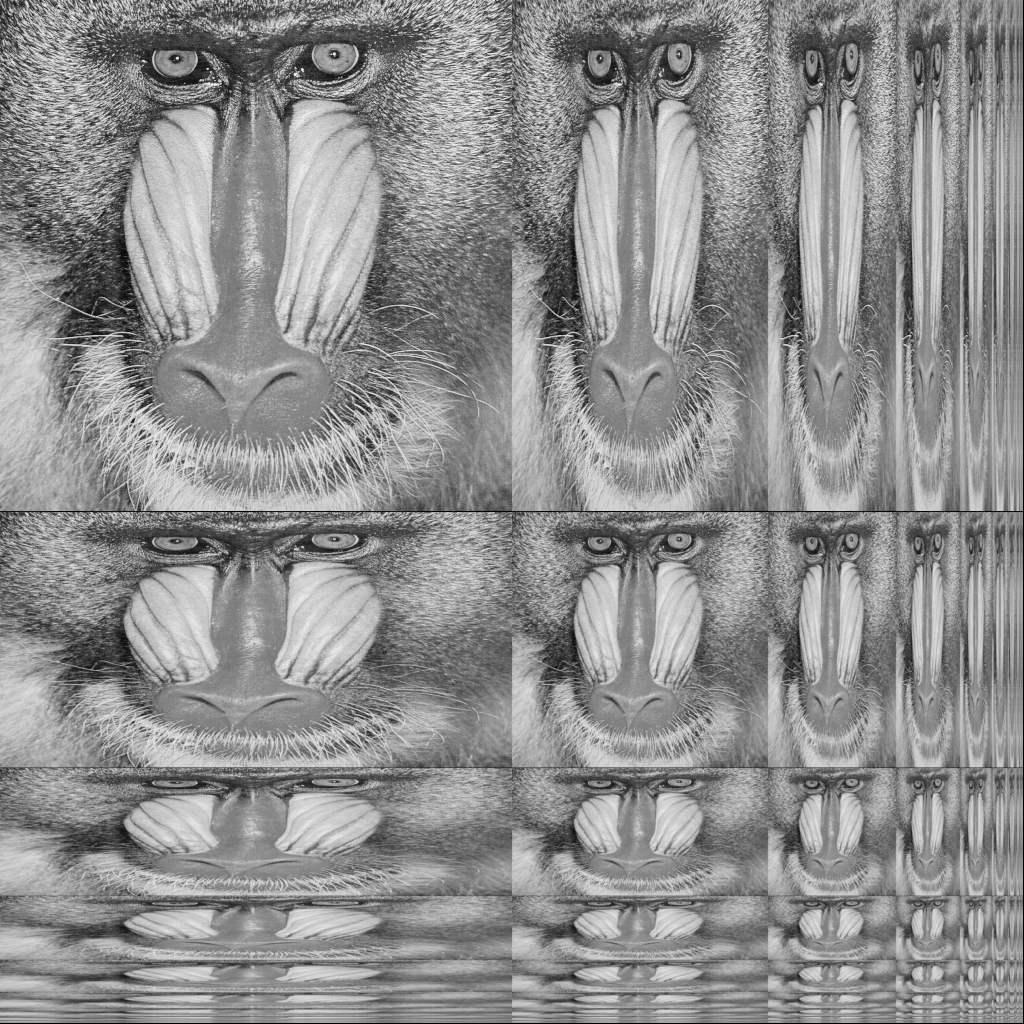
\includegraphics[scale=0.4]{Ripmap_real}
\caption{An example of Ripmap (cf. partie \ref{label_figure_Ripmap_jt})}
\label{Ripmap_real}
\end{figure}


\label{label_schema_interp_quadrilin_jt}
\begin{figure}[h!]
\centering
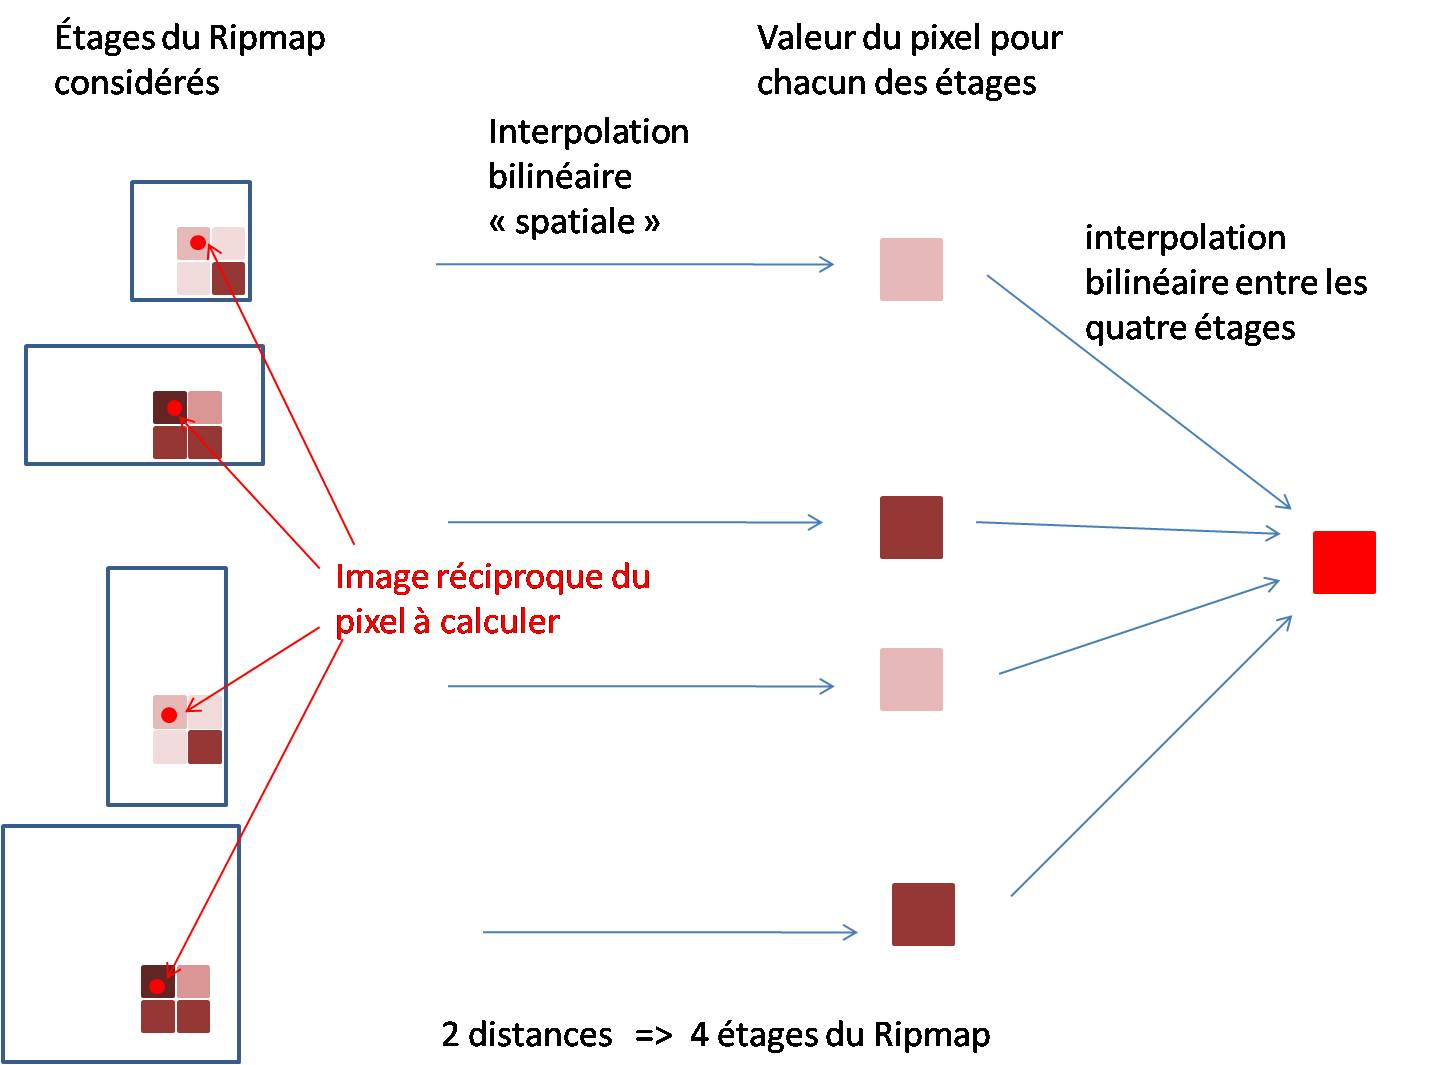
\includegraphics[scale=0.5]{interbibilineaire.jpg}
\caption{Quadri-linear (cf. section \ref{label_schema_interp_quadrilin_jt})}
\label{interbibilineaire}
\end{figure}

The parallelogram is approximated by the smallest rectangle in which it is contained, so the distance function is defined by

%On a utilisé le plus petit rectangle qui contient le parallélogramme. Ainsi la formule est :
$$D(x,y) = \left( \left|\frac{\dr u}{\dr x}\right|+\left|\frac{\dr u}{\dr y}\right|,\left|\frac{\dr v}{\dr x}\right|+\left|\frac{\dr v}{\dr y}\right|\right)$$

and the point considered has been translated in order for the rectangle to contain the parallelogram, as seen in the figure  \ref{methode_distance_ripmap}.

%On a de plus décalé les points pour que le rectangle considéré soit bien celui qui contient le parallélogramme, comme on le voit sur la figure \ref{methode_distance_ripmap}.

\label{label_meth_petit_rect_jt}
\begin{figure}[h!]
\centering
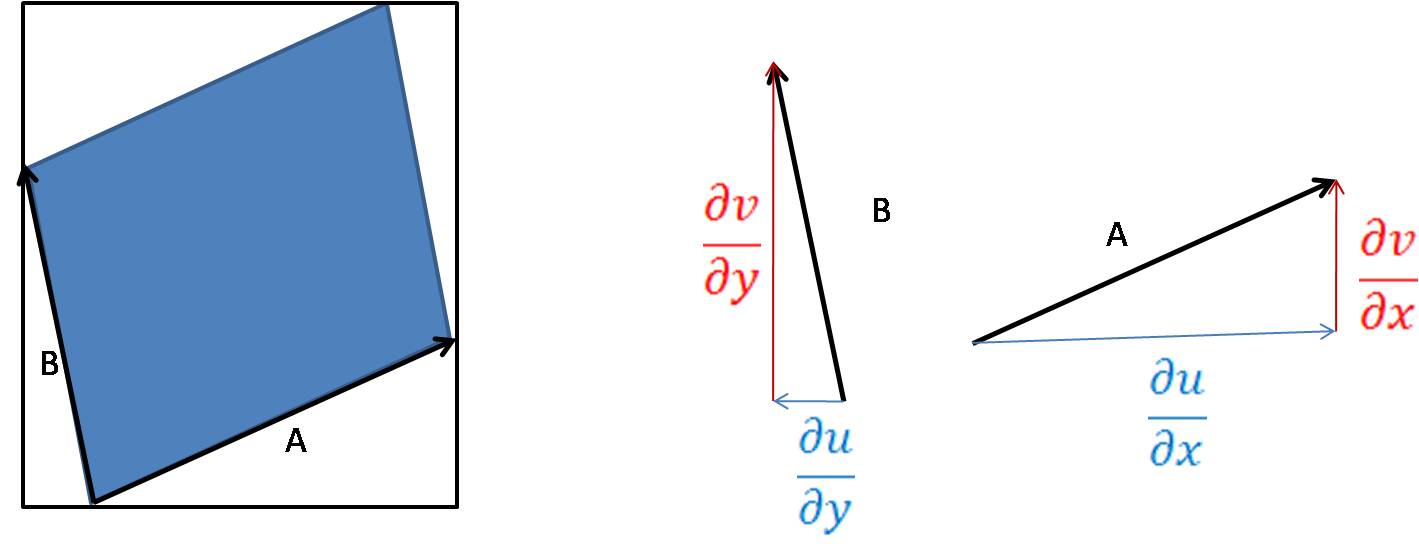
\includegraphics[scale=0.5]{methode_distance_ripmap.jpg}
\caption{Smallest rectangle method for the Ripmap (cf. section \ref{label_meth_petit_rect_jt})}
\label{methode_distance_ripmap}
\end{figure}

The algorithm for the Ripmap is describe in section \ref{pseudo_code_Ripmap}.

It is an improvement of the Mipmap, but it does not solve for instance the case of a thin rectangle in diagonal.

%On peut consulter le pseudo-code pour le Ripmap en section \ref{pseudo_code_Ripmap}.

%Cela améliore certes la méthode, mais ne résout pas par exemple le cas d'un rectangle fin en diagonale.
